%!TEX root = ../thesis.tex
%Adding the above line, with the name of your base .tex file (in this case "thesis.tex") will allow you to compile the whole thesis even when working inside one of the chapter tex files

\singlespacing
\chapter{Coronal Mass Ejection Shocks and Particle Acceleration} 
\label{chap:5}

This chapter is based on work published in Carley et al., {\it Nature Physics}, 2013, and Zucca et al., {\it Astronomy \& Astrophysics}, submitted.

\doublespacing
\section{Introduction}\label{sec:1}
Coronal mass ejections (CMEs) are spectacular eruptions of magnetized plasma from the low solar atmosphere into interplanetary space \citep{byrne2010, roussev2012}. With kinetic energies of $\sim$$10^{25}$\,J \citep{vourlidas2010}, they are the most energetic explosive events in the solar system and are often associated with plasma shocks and the acceleration of particles to relativistic speeds \citep{klassen2002, grechnev2011}. However, the underlying mechanism relating CMEs, shocks, and particle acceleration is still a subject of intense debate \citep{vrsnak2008}. By clarifying the inherent characteristics of these phenomena we learn not only about the nature of explosive plasma events but also about how they drive shocks and accelerate particles to high energies. Such processes are ubiquitous in the universe, playing a role in the acceleration of cosmic rays in supernovae and active galactic nuclei shocks \citep{drury2012}.


CME-associated shocks are often observed over a variety of spectral bands. At radio frequencies, high intensity ($\sim$$10^8$\,Jy) emissions, known as type II and type III bursts, are associated with coronal shocks and accelerated particles in the solar corona \citep{wild1950, mann1996}. Fine structure in these radio bursts can often reveal a \textquoteleft bursty' nature to the shock particle acceleration \citep{mann2005}, which can reveal details of the internal shock structure \citep{zlobec1993, guo2010}.
At extreme ultraviolet (EUV) wavelengths, the shock or pressure pulse response of the corona to an eruption may be imaged as a bright pulse propagating across the entire solar disk at typical velocities of 200--400\,km\,s$^{-1}$ \citep{gallagher2011}. These \textquoteleft coronal bright fronts' (CBFs) are a regular feature of solar eruptive events and often display wave-like properties such as reflection \citep{gopal2009}, refraction \citep{wang2000} and pulse broadening \citep{long2011}. %
Like CMEs, CBFs are often accompanied by type II and type III radio bursts, with EUV and radio images revealing a spatial link between the phenomena that is suggestive of a common origin \citep{maia2004, kozarev2011, vrsnak2005}.


It has been proposed that the common origin for these myriad phenomena may be a CME-driven shock \citep{grechnev2011, warmuth2004b}.  In this scenario, the CME eruption drives a pressure pulse, observable in the low corona as a propagating wave-like CBF. Higher in the corona this same pulse forms a shock, accelerating particles and producing type II and III emission. However, much debate surrounds the suggestion that (i) the CBF is a plasma pressure wave driven by a CME, and (ii) the radio bursts, generated by accelerated particles, result from this same wave/shock system. The contention has arisen from attempts to explain non-wave kinematics of CBFs \citep{zhukov2009}. Pseudo-wave theories are employed to describe this behavior, where the erupting CME produces a large-scale restructuring of the coronal magnetic field, which results in a propagating bright pulse (via Joule plasma heating) that is not actually a driven wave \citep{delannee2008}. In this scenario, any relationship with shock observables is indirect. Further confusion is added by the possibility that high energy particles in association with the eruption may be a consequence of magnetic reconnection in the flaring active region, and not the result of a shock \citep{kahler2007}.

Collectively, CMEs, CBFs and radio bursts provide direct measures of both shock kinematics and the characteristics of the accompanying accelerated particles. However, a common theory explaining these phenomena has yet to be verified.
This lack of clarity can be ascribed to an EUV imaging cadence that was unable to match the fast time sampling of radio imaging and spectroscopy. Now, using the high image cadence of the Solar Dynamics Observatory \citep[SDO;][]{presnell2012}, combined with fast time sampling radio images and spectra, we can reveal previously unseen characteristics of the relationship between these phenomena, proving that a CME-driven shock is the feature unifying these observations and that this shock is responsible for bursty electron acceleration. This greatly advances our understanding of the close relationship between solar eruptions, plasma shocks and their resulting EUV, radio and particle acceleration signatures.


\subsection{Coronal Bright Front and Radio Source}\label{sec:10}

\begin{sidewaysfigure}
    \centering
	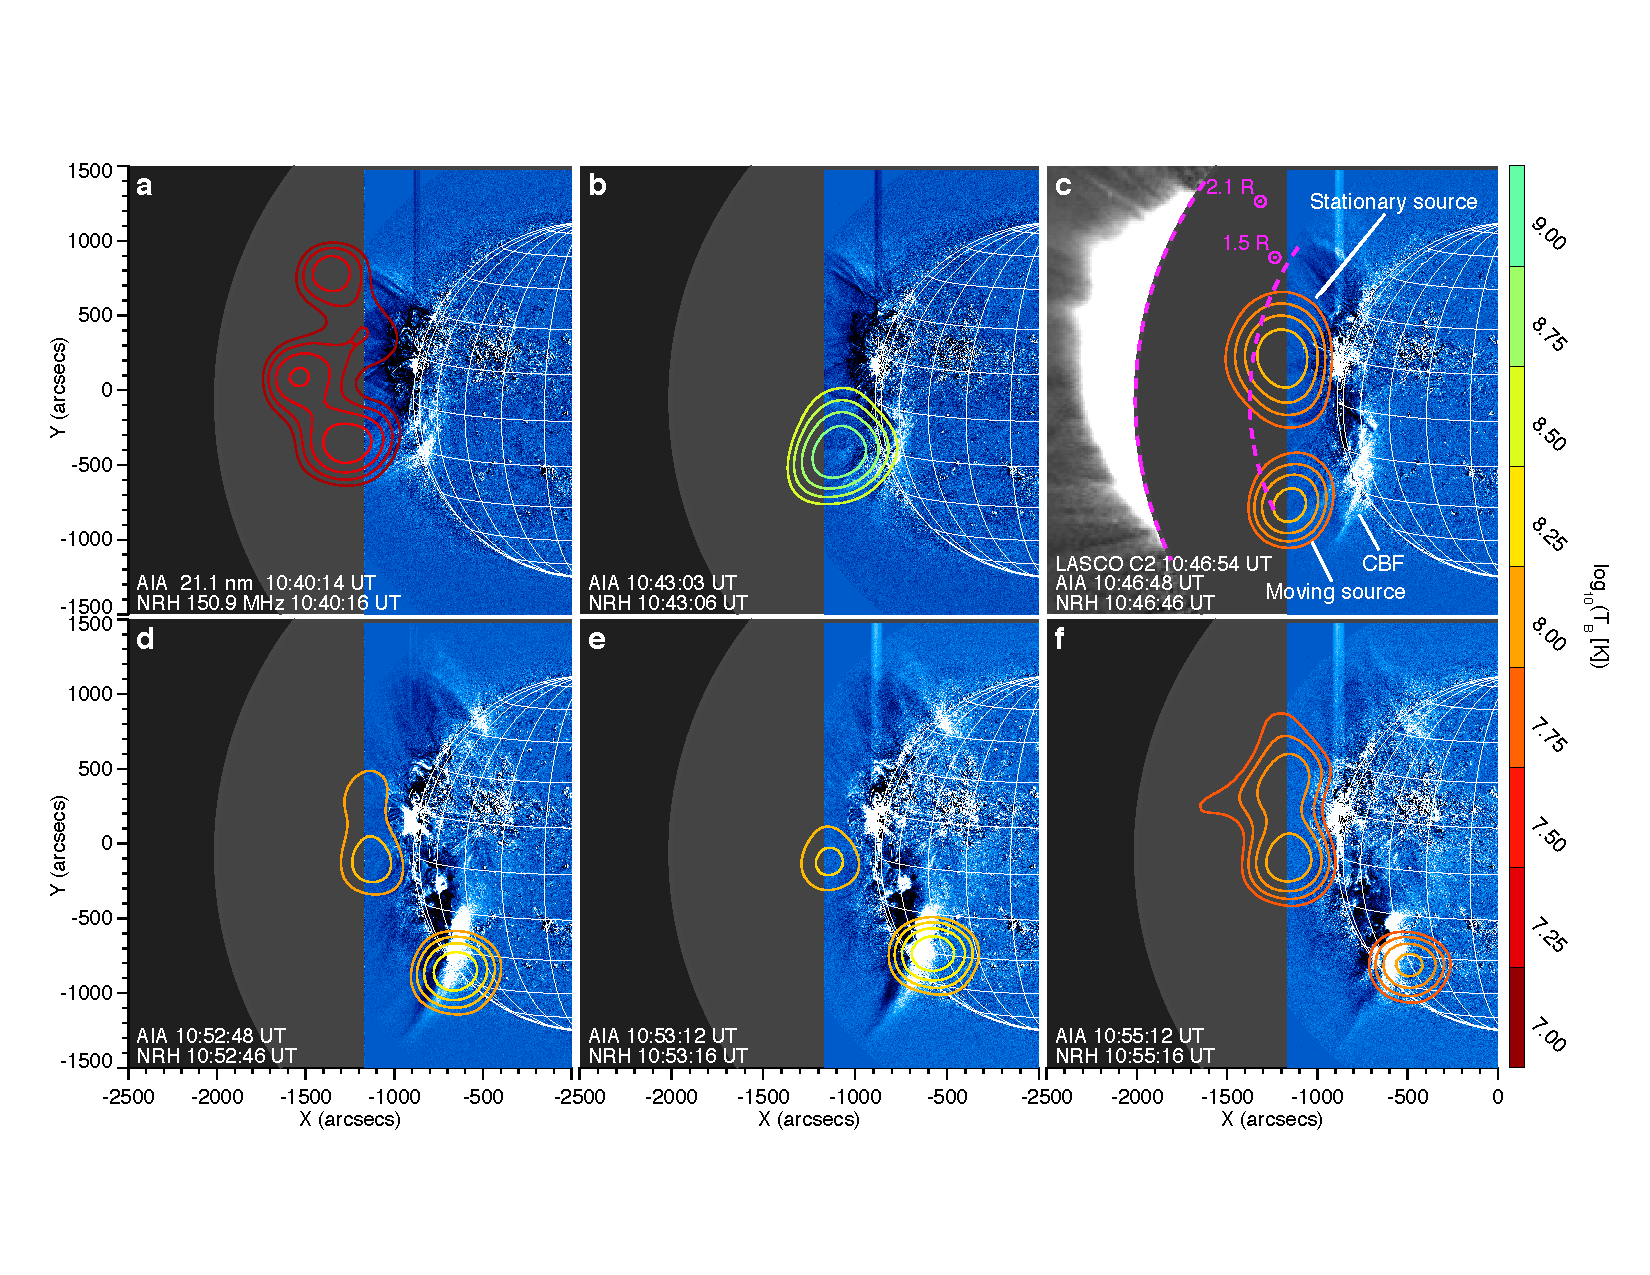
\includegraphics[scale=0.8, trim=0cm 2cm 0cm 0cm]{gallagher_figure1_final.pdf}
	\caption{Caption}
	\label{fig:cbf_radio_source}
\end{sidewaysfigure}


\subsection{Radio Dynamic Spectra}\label{sec:20}


\subsection{Relationship Between CME, CBF, and Radio bursts}\label{sec:31}


